\documentclass{article}

\usepackage[utf8]{inputenc}
\usepackage[english]{babel}
\usepackage[%
    left=1.30in,%
    right=1.30in,%
    top=1.0in,%
    bottom=1.0in,%
]{geometry}%
\usepackage{float}
\usepackage{amsfonts}
\usepackage{mathtools}
\usepackage{graphicx}
\usepackage{csquotes}
\usepackage{biblatex}
\usepackage{tikz}
\usepackage[colorlinks=true]{hyperref}

\addbibresource{bibliography.bib}
\graphicspath{ {./images/} }

\newcommand{\defeq}{
    \stackrel{def}{=}
}
\newcommand{\tablegraphics}[2]{
    \raisebox{-.5\height}{\includegraphics[scale=#2]{#1}}
}
\DeclarePairedDelimiter{\norm}{\lVert}{\rVert}
\usetikzlibrary{positioning,arrows.meta,calc,fit}
\def\trapW{3}
\def\trapHa{.9}
\def\trapHb{2}
\def\borderW{0.2mm}
\def\imgscl{.7}
\def\lrgimgscl{.5}

\newcommand{\recfigfragment}[7]{
    \textbf{#1} & \tablegraphics{#2/#3}{\imgscl} & \tablegraphics{#2/#4}{\imgscl} & \tablegraphics{#2/#5}{\imgscl} & \tablegraphics{#2/#6}{\imgscl} & \tablegraphics{#2/#7}{\imgscl}
}

\newcommand{\recfig}[5]{
    \begin{figure}[H]
    \centering
    \bgroup
    \def\arraystretch{4}
    \begin{tabular}{c c c c c c}
    \hline\hline
    \recfigfragment{Original images}{frogs}{frog-#1}{frog-#2}{frog-#3}{frog-#4}{frog-#5} \\
    \hline
    \recfigfragment{GLO}{glototalrec}{#1-fake}{#2-fake}{#3-fake}{#4-fake}{#5-fake} \\
    \hline
    \recfigfragment{Our (without term)}{ournopertrec}{#1-fake}{#2-fake}{#3-fake}{#4-fake}{#5-fake} \\
    \hline
    \recfigfragment{Our (with term)}{ourrec}{#1-fake}{#2-fake}{#3-fake}{#4-fake}{#5-fake} \\
    \hline\hline
    \end{tabular}
    \setlength{\tabcolsep}{5em}
    \egroup
    \caption{A few reconstructions of training images}
    \end{figure}
}

\newcommand{\encrecfig}[6]{
    \begin{figure}[H]
    \centering
    \bgroup
    \def\arraystretch{4}
    \begin{tabular}{c c c c c c}
    \hline\hline
    \recfigfragment{Original images}{frogs}{frog-#1}{frog-#2}{frog-#3}{frog-#4}{frog-#5} \\
    \hline
    \recfigfragment{Reconstructed}{encrec}{#1-fake}{#2-fake}{#3-fake}{#4-fake}{#5-fake} \\
    \hline\hline
    \end{tabular}
    \setlength{\tabcolsep}{5em}
    \egroup
    \caption{A few reconstructions of #6 images}
    \end{figure}
}

\newcommand{\interfig}[4]{
    \begin{figure}[H]
    \centering
    \bgroup
    \def\arraystretch{5}
    \begin{tabular}{c c}
    \hline\hline
    \textbf{GLO} & \tablegraphics{glototalinter/#1-#2n}{\lrgimgscl} \\
    \hline
    \textbf{Our (without term)} & \tablegraphics{ournopertinter/#1-#2n}{\lrgimgscl} \\
    \hline
    \textbf{Our (with term)} & \tablegraphics{ourinter/#1-#2n}{\lrgimgscl} \\
    \hline\hline
    \end{tabular}
    \setlength{\tabcolsep}{5em}
    \egroup
    \caption{An interpolation of #4 images (#3)}
    \end{figure}
}
\tikzset
{
  Trapezium/.pic =
  {
    \draw [line width=\borderW] (0,0) -- (0,\trapHa) -- (\trapW,\trapHb) -- (\trapW,-\trapHb) -- (0,-\trapHa) -- cycle ;
    \coordinate (-center) at (\trapW/2,0);
    \coordinate (-out) at (\trapW,0);
  },
  Arrow/.style=
  {
    line width=2mm,
    -{Triangle[length=2.5mm,width=5mm]},
    shorten >=2pt,
    shorten <=2pt,
  }
}
\newcommand{\EncoderDecoder}{
\begin{figure}[H]
\centering
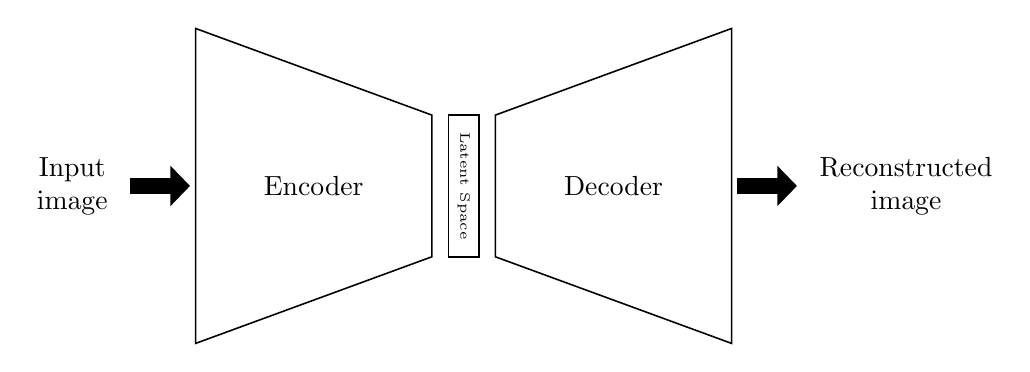
\begin{tikzpicture}
[
  node distance=2mm, % space between drawn parts
  every node/.style={align=center},
]
\node (latSpace) 
  [
    draw,
    line width=\borderW,
    minimum height=2*\trapHa cm,
    font=\tiny,
  ]
  {\rotatebox{-90}{Latent Space}};
  \pic (left)[left=of latSpace.west, rotate=180] {Trapezium};
  \pic (right)[right=of latSpace.east] {Trapezium};
  \node at (left-center) {Encoder};
  \node at (right-center) {Decoder};
  
  \def\d{.9}
  \coordinate (u) at (\d,0);
  \draw [Arrow] (right-out) -- ++(u) node [anchor=west] {Reconstructed\\image};
  \draw [Arrow] ($(left-out)-(u)$) node [anchor=east] {Input\\image} -- ++(u) ;
\end{tikzpicture}
\caption{Illustration of the architecture}
\end{figure}
}

\title{Improving the GLO learning process}
\author{Yuval Helman, Jakov Zingerman, Ran Schreiber}
\date{Tel Aviv University, August 2019}

\begin{document}
\maketitle

\section{Introduction}
Unconditional image generation is the task of learning a mapping from a space, called the \textit{latent space}, to an infinite image domain, by only looking at a finite subset of this domain. This mapping is the desired generator, we may randomly select a latent vector and use the mapping to synthesize an image from our image domain.  A highly important property of the generating function, which is necessary for tasks that perform operations in the latent space (e.g. image interpolation), is that euclidean distances between latent vectors would be mapped to perceptually and semantically meaningful differences in the image space. Its private case of mapping interpolations of latent vectors into semantic interpolations in the image space is referred to as \textit{continuity} in this report.

Image generators are useful for a variety of applications. They may be used for synthesizing new training images in cases where data is either lacking or too expensive, as medial data usually is \cite{frid2018synthetic, shin2018medical}; Such data is necessary for other machine-learning tasks, such as classification. In addition, image generators may be a fundamental building block for other algorithms; For example, the \textit{NAM} algorithm by Hoshen and Wolf that learns an unconditional mapping between two image domains relies on the existence of a generator for the target domain \cite{hoshen2018nam}.

\subsection{Generative adversarial networks (GAN)}
The task of image generation may be solved very well using \textit{GAN}, in which two neural networks are simultaneously trained - one is the \textit{generator}, and the second is the \textit{discriminator} which estimates the authenticity of its input images \cite{goodfellow2014generative}. However, \textit{GAN}s are somewhat problematic. They are commonly very hard to train because the training process is usually highly sensitive to the choice of hyperparameters, which are the parameters that are not trained but are set manually; In addition, in most cases multiple initializations of the weights are required for gaining a fine generator because of the \textit{mode collapse} phenomenon, in which the generator produces samples only from a few parts, called "modes", of the data distribution. These disadvantages have motivated researchers to find non-adversarial alternatives for the task of image generation.

\subsection{Generative Latent Optimization (GLO)}
\label{sec:sec1.2}
One of the most effective non-adversarial algorithms for the task is \textit{GLO} by Bojanowski et al \cite{bojanowski2017optimizing}. As our proposed method is based on it, we will present it briefly.

Let us denote the training set by $S$; In order to find the generating function $G$, the algorithm finds an optimal latent vector $z_x$ from a predefined latent space $\mathcal{Z}$ (in this project we define it to be $\mathbb{R}^d$ where $d$ is its dimension) for each sample $x$ in the training set. That is, the algorithm jointly learns the latent vectors $\{z_x\}_x$ and the weights of the neural network $G$. The objective is given by this formula:

$$\arg{\min_{G,\{z_x\}_{x \in S}} \sum_{x \in S} loss(G(z_x), x)} \qquad s.t. \{z_x\}_{x \in S} \subset \mathcal{Z}$$
The aforementioned $loss$ is a weighted combination of the \textit{Laplacian Pyramid Loss} and the $l_2$ loss; It compares how two given images are different.

Although the \textit{GLO} algorithm is very effective, it has a few shortcomings. The algorithm maintains a latent vector for each image in the training set, and as the set is used altogether during the training process and is not split, the optimization is done over millions of parameters. We believe that it makes the training process much more difficult.

In addition, a major downside of the algorithm is the absence of a trained inverse mapping from the image domain to the latent space; Such a mapping is necessary for tasks that perform operations in the latent space. If the input image for such a task is taken from the training set, the \textit{GLO} algorithm returns its optimal latent vector, and we are done; However, in the general case, we need to find its latent vector by performing a new optimization process: We define the latent vector $z$ of the input image $x$ to be $\arg{\min_z loss(G(z), x)}$, where $loss$ may be any function that compares how two images are different. This optimization makes the task extremely slow, and also unreliable since the objective is highly non-convex.

\section{Our Method}
Our method is based on the \textit{GLO} algorithm and tries to improve it - we want it to train both a generator and its inverse mapping, and we want the learning process to be more effective. That is, we want it either to be faster or to achieve more pleasing results in the same training time.

The algorithm is comprised of several stages; we first present the whole process briefly and then discuss each stage in detail. First, the training set is split to some predefined number of subsets; Then, there is a sequence of stages, each one is a modified \textit{GLO} algorithm that focuses on a small portion of the training set; Thereafter, a modified \textit{GLO} algorithm that deals with the whole training set is run. Finally, An inverse mapping model from the image domain to the latent space is trained.

Our algorithm trains two neural networks - an \textit{encoder}, which is a mapping from the image domain to the latent space, and a \textit{decoder}, which is a mapping from the latent space to the image domain.

\EncoderDecoder

The \textit{decoder} network, which functions as a generator, is trained in a few stages; Each stage, excluding the last one, involves a relatively small number of images, and thus a relatively small number of parameters that should be learned. We call this notion \textit{incremental learning}, and we believe it may lead to a much more effective training process.

The algorithm has a geometric intuition: the image space may be viewed as a smooth manifold, and the \textit{decoder} may be viewed as a parameterization of this manifold; the algorithm incrementally builds the image space - it starts by learning well a small number of points on the manifold (these points should be scattered so they "cover" the manifold as good as much as possible), then it learns other points, and so forth; Overall, the manifold is built incrementally.

\subsection{Splitting the training data}
As explained, each subset should "cover" as possible the image space. For achieving this, we perform a multistage process: We first cluster the whole training set to some predefined number of clusters; Next, we select a few representatives from each cluster to be the first set of images (the number of representatives is also predefined); Then we perform these two stages (clustering and selecting representatives) iteratively - each time using the images not selected in the previous stages - and eventually all the remaining images form the last set of images. This sequence of stages yields a sequence of disjoint sets whose union is the whole training set, and the images in each set are perceptually different.

For clustering a set of images we follow the \textit{ResNet Classifier Clustering} proposed by Sage et al. \cite{sage2018logo}: The last pooling layer of a \textit{ResNet-50} network pretrained on the \textit{ImageNet} dataset is used for extracting useful features of the images; These 2048-dimensional features are dimensionality reduced using the \textit{PCA} algorithm, and finally, we cluster the resulting vectors using the \textit{k-means} algorithm.

The $k$ representatives of each cluster of images are defined to be the $k$ images that correspond to the $k$ dimensionality reduced feature vectors that are nearest to the cluster's centroid (which is the mean of the points that form the cluster); The representatives are calculated using the \textit{k-nearest neighbors} algorithm.

\subsection{Modified GLO Algorithms}
The \textit{GLO} algorithm is run in three different variants in our algorithm - the first is run at the first stage involving a \textit{GLO} algorithm (that is, the first stage after splitting the data), the second is run at all of the intermediate stages and the third is run at the last stage involving a \textit{GLO} algorithm using the whole training set.

\subsubsection{The first variant}
The first variant of the algorithm involves the first subset of the training data and is identical to the original \textit{GLO}, except for using the \textit{VGG Perceptual Loss} instead of a weighted combination of the \textit{Laplacian Pyramid Loss} and the $l_2$ loss. This loss has been shown to estimate the perceptual similarity between two images in a way that approximately coincides with human judgment \cite{zhang2018unreasonable}, and is given by this formula:

$$ \norm{x, y}_{VGG} \defeq \norm{x - y}_1 + \sum_i \norm{\phi_i (x) - \phi_i (y)}_1$$
$\norm{\cdot}_1$ is the $l_1$ norm; $\phi_i(\cdot)$ is the vector of features that is extracted at the end of the ith block of a \textit{VGG} network pretrained on the \textit{ImageNet} dataset.

\subsubsection{The second variant}
The second variant of the algorithm focuses on one subset of the training data while trying to preserve the results of the previous stages. That is, let $n \leq 2$ be the total number of subsets obtained in the first stage of the algorithm. The first subset is processed by the first \textit{GLO} variant described above; For each $1 < i \leq n$ there is a corresponding stage in the algorithm which focuses on it and tries to preserve the results of the previous stages (which trained the first $i-1$ subsets).

It is done as follows: Let us denote the subsets already trained by $S_p$ ($p$ denotes "previous"), and the subset we focus on by $S_c$ ($c$ denotes "current"); The algorithm finds an optimal latent vector $z_x$ for each sample $x$ in $S_c$, and tries to preserve the good \textit{decoder}'s reconstruction of $S_p$ (which has been obtained in the previous stages). That is, the algorithm jointly learns the latent vectors $\{z_x\}_{x \in S_c}$ and the weights of the neural network $G$; Of course, these weights are initialized with the learned values calculated in the previous stage. The objective is given by this formula:

$$\arg{\min_{G,\{z_x\}_{x \in S_c}} \alpha \cdot \bigg(\sum_{x \in S_p} \norm{G(z_x), x}_{VGG}\bigg) + \beta \cdot \bigg(\sum_{x \in S_c} \norm{G(z_x), x}_{VGG}\bigg)}$$
For each $x \in S_p$, $z_x$ has been calculated in the previous stage and is now fixed; $\alpha$ and $\beta$ are hyperparameters which control the significance of each term in the loss function.

\subsubsection{The third variant}
The third variant of the algorithm involves the complete training set. As in the first variant, the algorithm finds an optimal latent vector for each sample in the training set, but now there is a new term in the loss function which should improve the continuity of the \textit{decoder}. Let us denote the training set by $S$, the objective is given by this formula:

$$\arg{\min_{G,\{z_x\}_{x \in S}} \alpha \cdot \bigg(\sum_{x \in S} \norm{G(z_x), x}_{VGG}\bigg) + \beta \cdot \bigg(\sum_{x \in S} \norm{G(z_x+\varepsilon(\sigma)), x}_{VGG}\bigg)}$$
$\alpha$, $\beta$ and $\sigma$ are hyperparameters, $\varepsilon(\cdot)$ is a normally distributed random variable with zero mean and variance $\sigma ^ 2$.


\subsection{Training an Encoder network}
After training a \textit{decoder}, an \textit{encoder} is trained as follows: Let us denote the training set by $S$, the objective is given by this formula:

$$\arg{\min_{E}} \ \sum_{x \in S} loss(E(x), z_x)$$
For each $x \in S$, $z_x$ is the optimal latent vector which has been calculated in the training process of the \textit{decoder}; The loss function used is a weighted combination of the $l_1$ and $l_2$ loss functions.

\section{Experiments}
We have conducted several experiments to estimate our algorithm; We have trained a \textit{GLO} model (to which we would compare our models), we have trained our \textit{decoder} without the loss term regarding the generator's continuity (we set its coefficient to zero), and we have trained our \textit{decoder} with this term. Afterward, we have trained an \textit{encoder} matching the \textit{decoder} with the additional loss term.

\begin{figure}[h]
\centering
\begin{tabular}{ c c }
  \hline\hline
  \textbf{Model} & \textbf{Training time} (h:m) \\ \hline
  GLO model & 09:27 \\ \hline
  Decoder without the additional loss term & 09:05 \\ \hline
  Decoder with the additional loss term & 08:59 \\ \hline
  Encoder & About 01:30 \footnotemark \\
  \hline\hline
\end{tabular}
\caption{The training time of the different models}
\end{figure}

\footnotetext{5000 epochs have been run in 6 hours and 41 minutes, but the optimum has been achieved at the epoch #1161; Therefore the training time is approximately 1.5 hours.}

\subsection{The dataset}
The dataset we have used is Jon Shamir's frogs dataset which consists of almost eight thousand 64*64 images \cite{shamirfrogsgit}. The first six thousand images have been used as a training set, and the remaining ones as a testing set; We haven't applied any data augmentation methods.

\begin{figure}[H]
\centering
\begin{tabular}{ c c c c }
 \tablegraphics{frogs/frog-18}{\imgscl} & \tablegraphics{frogs/frog-183}{\imgscl} & \tablegraphics{frogs/frog-197}{\imgscl} & \tablegraphics{frogs/frog-321}{\imgscl} \\
 \tablegraphics{frogs/frog-349}{\imgscl} & \tablegraphics{frogs/frog-4759}{\imgscl} & \tablegraphics{frogs/frog-7786}{\imgscl} & \tablegraphics{frogs/frog-229}{\imgscl} \\
\end{tabular}
\caption{A few samples from the dataset}
\end{figure}

As may be seen, the dataset is quite diverse - the frogs vary in their colors, shapes, sizes, and positions.

\subsection{Implementation details}
The repository of the project is available on Github \footnotemark ; It contains all the training and evaluation source files, bash scripts for settings up the environment, different trained models and the results of the experiments conducted. The code is based on the \textit{PyTorch}, \textit{NumPy}, \textit{Matplotlib}, \textit{scikit-learn} and \textit{scikit-image} libraries in \textit{Python 3.7}.

\footnotetext{\url{https://github.com/ransch/MLApplicationsForGraphics/}}

The dimension of the latent space used in the experiments is $100$; The \textit{decoder} network used is the generator of the \textit{DCGAN} architecture \cite{radford2015unsupervised}; The \textit{encoder} network used is a variant of the discriminator of the \textit{DCGAN} architecture - instead of the sigmoid layer in the end, we have a linear layer; The optimization algorithm used is Adam \cite{kingma2014adam}.

\subsection{Reconstructing training images}
The images in the training set have been reconstructed both by a generating function learned using the \textit{GLO} algorithm, and by a generating function learned using our algorithm: The reconstruction of an image $x$ from the training set is defined to be $G(z_x)$, where $G$ is the learned generator and $z_x$ is the optimal latent vector of $x$ that the algorithm computes.

The first row of Figure 3 presents a few frogs images from the training dataset, the second presents their reconstructions using a \textit{GLO} model, the third presents the reconstructions using our model without the loss term regarding the generator's continuity, and the last row presents the reconstructions using our model including this loss term.

\recfig{168}{170}{250}{8}{9}

Our method hasn't achieved more pleasing results than the \textit{GLO} algorithm; An interpretation of the results and proposed further work may be found at the \hyperref[sec:sec4]{Discussion} Section.

\subsection{Interpolating training images}
Reconstructions of training images have been interpolated both by a \textit{GLO} model and by our model: Given two images $x$ and $y$, we take their optimal latent vectors $z_x$ and $z_y$ (computed by the algorithm), split the interval between them to some desired number of points, and apply the learned generating function to each one of these points.

The first row in each section in Figures 4-6 presents an interpolation done by a \textit{GLO} model, the second presents an interpolation done by our model without the loss term regrading the generator's continuity, and the third presents an interpolation done by our model including this loss term. More interpolations may be found at the end of the report.

\interfig{1113}{1114}{i}{training}
\interfig{1207}{1234}{ii}{training}
\interfig{1246}{1247}{iii}{training}

As can be seen, the interpolations done by our models (both with the loss term regarding the generator's continuity and without it) are perceptually more pleasing than the ones that are done by a \textit{GLO} model. By looking at the interpolations done by the \textit{GLO} model, it seems that the generating function is quite non-continuous, while our models appear to be much more continuous. Moreover, the model which includes the additional loss term seems to interpolate better than the one which doesn't include it.

\subsection{Encoding training images}
Images from the training set have been reconstructed using an \textit{encoder} and a \textit{decoder}: The reconstruction of an image $x$ is defined to be $D(E(x))$, where $D$ is the learned \textit{decoder} (that is, the learned generator) and $E$ is the learned \textit{encoder}. The \textit{decoder} used is the one which has been trained using the additional loss term (regarding the continuity).

\encrecfig{37}{331}{459}{600}{623}{training} 

As can be seen, the results are yet to be satisfactory with the acquired model - the images have no texture and are blurry. Again, we interpret and propose further work at the \hyperref[sec:sec4]{Discussion}.

\subsection{Encoding test images}
Images from the test set have been reconstructed using an \textit{encoder} and a \textit{decoder}; The \textit{decoder} used is the one which has been trained using the additional loss term (regarding the continuity).

\encrecfig{7203}{7215}{7667}{7772}{7787}{testing}

\section{Discussion}
\label{sec:sec4}
In this project, we have tried to improve the \textit{GLO} algorithm by dealing with its downsides discussed above (\hyperref[sec:sec1.2]{Section 1.2}). As can be seen, The \textit{encoder} has not been trained satisfactorily yet; There may be several reasons for this - the network's architecture might not fit well, and maybe the network should be trained jointly with the \textit{decoder}, and not separately. In addition, our models haven't achieved more pleasing reconstructions of training images than the \textit{GLO} model. However, we have seen that both the notion of \textit{incremental learning} and the additional loss term succeed in improving the quality of the trained \textit{decoder} as it seems to be more continuous.

It may be interesting to repeat the experiments conducted with a different choice of the latent space $\mathcal{Z}$, and to adapt the \textit{GLANN} algorithm by Hoshen and Malik \cite{hoshen2019non} (which is based on \textit{GLO} and outperforms it) to our method. 

\section{Additional Interpolation Comparisons}
\interfig{1568}{1574}{iv}{training}
\interfig{1779}{1780}{v}{training}

\bigskip
\newrefcontext[sorting=nyt]
\printbibliography[heading=bibnumbered]
\bigskip

\end{document}